\documentclass[aspectratio=169]{beamer}

\usetheme{Madrid}
\usecolortheme{seahorse}
\setbeamertemplate{navigation symbols}{}
\setbeamertemplate{footline}[frame number]

\usepackage{booktabs}
\usepackage{amsmath}
\usepackage{tikz}
\usepackage{listings}
\usepackage{xcolor}

\lstdefinestyle{lean}{
    basicstyle=\ttfamily\scriptsize,
    keywordstyle=\color{blue!70!black}\bfseries,
    commentstyle=\color{green!50!black},
    stringstyle=\color{red!60!black},
    showstringspaces=false,
    breaklines=true,
    frame=single,
    backgroundcolor=\color{gray!5},
    rulecolor=\color{gray!30},
}

\lstdefinestyle{python}{
    language=Python,
    basicstyle=\ttfamily\scriptsize,
    keywordstyle=\color{blue!70!black}\bfseries,
    commentstyle=\color{green!50!black},
    stringstyle=\color{red!60!black},
    showstringspaces=false,
    breaklines=true,
    frame=single,
    backgroundcolor=\color{gray!5},
    rulecolor=\color{gray!30},
}

\title{Mode Collapse in RL-Trained Theorem Provers}
\subtitle{Structural Guidance as a Diagnostic and Remedy}
\author{Zachary Burton}
\institute{arXiv: 2601.16172}
\date{}

\begin{document}

\begin{frame}
\titlepage
\end{frame}

%% ---- SLIDE 2: BACKGROUND ----
\begin{frame}{Background: Neural Theorem Proving}
\begin{columns}
\begin{column}{0.55\textwidth}
\textbf{Setup:}
\begin{itemize}
    \item Formal theorem $x$ in Lean 4 (dependent type theory)
    \item LLM $P_\theta$ generates tactic proof $y$
    \item Lean kernel verifies: $\text{check}(x, y) \in \{\top, \bot\}$
    \item Sample $k$ attempts, accept if any verify
\end{itemize}

\vspace{0.5em}
\textbf{State of the art:}
\begin{itemize}
    \item DeepSeek-Prover-V1.5-RL: 7B params, GRPO-trained
    \item Combines SFT $\to$ RL with Monte-Carlo tree search
    \item Evaluated on miniF2F: 244 competition-level theorems
\end{itemize}
\end{column}
\begin{column}{0.4\textwidth}
\centering
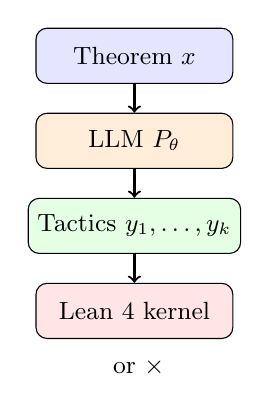
\begin{tikzpicture}[
    box/.style={draw, rounded corners, minimum width=2.5cm, minimum height=0.7cm, align=center, font=\small},
    scale=0.9
]
    \node[box, fill=blue!10] (thm) at (0, 3) {Theorem $x$};
    \node[box, fill=orange!15] (llm) at (0, 1.8) {LLM $P_\theta$};
    \node[box, fill=green!10] (tac) at (0, 0.6) {Tactics $y_1, \ldots, y_k$};
    \node[box, fill=red!10] (lean) at (0, -0.6) {Lean 4 kernel};
    \node[font=\small] at (0, -1.4) {$\checkmark$ or $\times$};
    \draw[->, thick] (thm) -- (llm);
    \draw[->, thick] (llm) -- (tac);
    \draw[->, thick] (tac) -- (lean);
\end{tikzpicture}
\end{column}
\end{columns}
\end{frame}

%% ---- SLIDE 3: THE PROBLEM ----
\begin{frame}{The Problem: Sampling Saturates Early}

\textbf{Standard assumption:} Pass@$k$ increases monotonically with $k$.

\vspace{0.5em}
\begin{columns}
\begin{column}{0.5\textwidth}
\begin{table}
\centering
\begin{tabular}{lc}
\toprule
\textbf{Budget} & \textbf{Theorems solved} \\
\midrule
$k = 16$ & 38 / 244 ~(15.6\%) \\
$k = 32$ & 42 / 244 ~(17.2\%) \\
$k = 64$ & \textbf{42 / 244 ~(17.2\%)} \\
\bottomrule
\end{tabular}
\caption*{\small DeepSeek-Prover-V1.5-RL, i.i.d.\ $T{=}0.6$}
\end{table}

\vspace{0.3em}
32 additional samples at $k{=}64$: \textbf{zero new proofs}.
\end{column}
\begin{column}{0.45\textwidth}
\centering
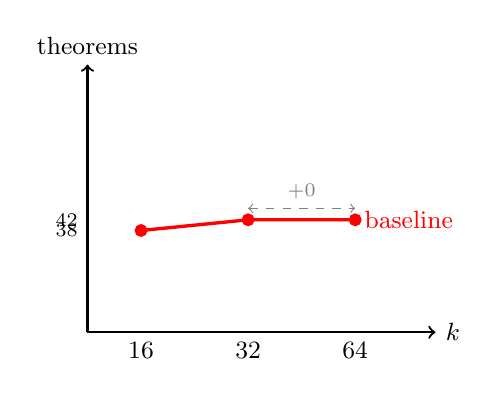
\begin{tikzpicture}[scale=0.85]
    \draw[->, thick] (0,0) -- (5.2,0) node[right] {\small $k$};
    \draw[->, thick] (0,0) -- (0,4) node[above] {\small theorems};
    % Baseline
    \draw[red, very thick, mark=*] plot coordinates {(0.8,1.52) (2.4,1.68) (4.0,1.68)};
    \node[red, font=\small] at (4.8,1.68) {baseline};
    % Ticks
    \node[below, font=\small] at (0.8,0) {16};
    \node[below, font=\small] at (2.4,0) {32};
    \node[below, font=\small] at (4.0,0) {64};
    % Y labels
    \node[left, font=\scriptsize] at (0,1.52) {38};
    \node[left, font=\scriptsize] at (0,1.68) {42};
    % Plateau annotation
    \draw[<->, gray, dashed] (2.4,1.85) -- (4.0,1.85);
    \node[gray, above, font=\scriptsize] at (3.2,1.85) {+0};
\end{tikzpicture}
\end{column}
\end{columns}

\vspace{0.5em}
\textbf{Hypothesis:} GRPO maximizes $\mathbb{E}[\text{reward}]$ per attempt, collapsing $P_\theta(y \mid x)$ onto a single high-probability strategy. Temperature sampling explores around this mode but cannot escape it.
\end{frame}

%% ---- SLIDE 4a: METHOD IDEA ----
\begin{frame}{Method: Expert Hints as Tactic Prefixes}

\textbf{Idea:} A student is stuck on a proof. You don't solve it---you say \emph{``have you tried induction?''} or \emph{``what if you simplify first?''}

\vspace{0.5em}
We encode this as a \textbf{tactic prefix} (skeleton) prepended to the model's prompt:

$$P_\theta(y \mid x, s) \quad \text{where } s \in \mathcal{S} \text{ is the hint}$$

\vspace{0.3em}
\begin{columns}[T]
\begin{column}{0.47\textwidth}
\textbf{Without hint:}
\begin{center}
\texttt{theorem T := by}\\
\texttt{~~\textcolor{gray}{<model generates>}}
\end{center}
$\to$ same strategy every time
\end{column}
\begin{column}{0.47\textwidth}
\textbf{With hint \texttt{ring}:}
\begin{center}
\texttt{theorem T := by}\\
\texttt{~~\textcolor{blue}{ring}}\\
\texttt{~~\textcolor{gray}{<model generates>}}
\end{center}
$\to$ forced into a different region of tactic space
\end{column}
\end{columns}

\vspace{0.5em}
\textbf{Key properties:} No retraining. No tree search. Deterministic schedule. Compatible with any completion-based prover.
\end{frame}

%% ---- SLIDE 4b: THE 15 SKELETONS ----
\begin{frame}{The 15-Skeleton Schedule}

We cycle through 15 common Lean tactics as prefixes (repeating for $k > 15$):

\vspace{0.5em}
\centering
{\small
\begin{tabular}{rlcrl}
\toprule
\textbf{\#} & \textbf{Skeleton} & \phantom{xx} & \textbf{\#} & \textbf{Skeleton} \\
\midrule
0 & (empty --- no hint) && 8 & \texttt{nlinarith} \\
1 & \texttt{simp} && 9 & \texttt{ring} \\
2 & \texttt{intro} && 10 & \texttt{ring\_nf} \\
3 & \texttt{intros} && 11 & \texttt{aesop} \\
4 & \texttt{constructor} && 12 & \texttt{refine $\langle$?\_,\,?\_$\rangle$} \\
5 & \texttt{refine ?\_} && 13 & \texttt{simp; try aesop} \\
6 & \texttt{norm\_num} && 14 & \texttt{simp; try nlinarith} \\
7 & \texttt{linarith} && & \\
\bottomrule
\end{tabular}
}

\vspace{0.5em}
\flushleft
Each skeleton represents a different high-level proof strategy: simplification, case splitting, algebraic normalization, arithmetic reasoning, etc.
\end{frame}

%% ---- SLIDE 5: CODE ----
\begin{frame}[fragile]{Implementation: Skeleton Injection}

\begin{columns}
\begin{column}{0.48\textwidth}
\textbf{IR definition} (\texttt{ir.py}):
\begin{lstlisting}[style=python]
TACTIC_SKELETONS = [
    (),              # empty
    ("simp",),
    ("intro",),
    ("intros",),
    ("constructor",),
    ("refine ?_",),
    ("norm_num",),
    ("linarith",),
    ("nlinarith",),
    ("ring",),
    ("ring_nf",),
    ("aesop",),
    ...
]

def perturb(base, seed, k, mode):
    for i in range(k):
        tactic = TACTIC_SKELETONS[
            i % len(TACTIC_SKELETONS)]
        yield IR(theorem=base.theorem,
                 tactic_prefix=tactic)
\end{lstlisting}
\end{column}
\begin{column}{0.48\textwidth}
\textbf{Prompt construction} (\texttt{search.py}):
\begin{lstlisting}[style=lean]
-- Standard (no skeleton):
theorem mathd_algebra_141 ... := by
  <model generates from here>

-- With skeleton "ring":
theorem mathd_algebra_141 ... := by
  ring
  <model generates from here>

-- With skeleton "simp", "try aesop":
theorem mathd_algebra_141 ... := by
  simp
  try aesop
  <model generates from here>
\end{lstlisting}

\vspace{0.3em}
{\small The skeleton is prepended to the completion prompt. The model sees it as context and continues from there.}
\end{column}
\end{columns}
\end{frame}

%% ---- SLIDE 6: CONCRETE EXAMPLES ----
\begin{frame}[fragile]{Concrete Examples: Skeletons Unlock New Proofs}

13 theorems solved \textbf{only} via skeletons (never by i.i.d.\ sampling):

\vspace{0.3em}
\begin{columns}
\begin{column}{0.48\textwidth}
\textbf{Example 1:} Prove $12 \mid 4^{n+1} + 20$

\vspace{0.2em}
{\scriptsize Without skeleton: model tries \texttt{norm\_num} variants, fails all 16.}

\vspace{0.2em}
Skeleton \texttt{simp} $\to$ model completes:
\begin{lstlisting}[style=lean]
theorem induction_12dvd4expnp1p20
  (n : N) : 12 | 4^(n+1) + 20 := by
  simp
  induction n with
  | zero => simp
  | succ n ih =>
    simp_all [Nat.mul_mod,
              Nat.pow_succ]
    omega
\end{lstlisting}

{\scriptsize The skeleton nudged the model toward \texttt{simp} + \texttt{induction} --- a strategy it never tried on its own.}
\end{column}
\begin{column}{0.48\textwidth}
\textbf{Example 2:} Given $ab{=}180$, $2(a{+}b){=}54$, show $a^2{+}b^2{=}369$

\vspace{0.2em}
{\scriptsize Without skeleton: model tries \texttt{field\_simp}, loops, fails.}

\vspace{0.2em}
Skeleton \texttt{ring} $\to$ model completes:
\begin{lstlisting}[style=lean]
theorem mathd_algebra_141
  (a b : R)
  (h1 : a * b = 180)
  (h2 : 2 * (a + b) = 54) :
  a^2 + b^2 = 369 := by
  ring
  nlinarith
\end{lstlisting}

\vspace{0.5em}
\textbf{Example 3:} Skeleton \texttt{aesop} $\to$ model chains\\
{\scriptsize \texttt{aesop <;> simp\_all <;> ring\_nf <;> norm\_num <;> linarith}}\\
{\scriptsize for an exponent manipulation problem it otherwise never solves.}
\end{column}
\end{columns}
\end{frame}

%% ---- SLIDE 7: MAIN RESULTS ----
\begin{frame}{Results: Skeletons Break the Plateau}

\begin{table}
\centering
\begin{tabular}{lccc}
\toprule
\textbf{Condition} & \textbf{Pass@16} & \textbf{Pass@32} & \textbf{Pass@64} \\
\midrule
A-RL: i.i.d.\ baseline & 38 ~(15.6\%) & 42 ~(17.2\%) & 42 ~(17.2\%) \\
\textbf{B-RL: skeleton schedule} & \textbf{55 ~(22.5\%)} & \textbf{58 ~(23.8\%)} & \textbf{60 ~(24.6\%)} \\
\midrule
Absolute gain & +17 & +16 & +18 \\
Relative gain & +44.7\% & +38.1\% & +42.9\% \\
\bottomrule
\end{tabular}
\end{table}

\vspace{0.3em}
\begin{columns}
\begin{column}{0.45\textwidth}
\centering
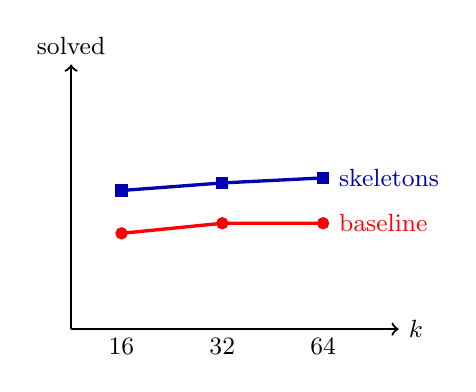
\begin{tikzpicture}[scale=0.8]
    \draw[->, thick] (0,0) -- (5.2,0) node[right] {\small $k$};
    \draw[->, thick] (0,0) -- (0,4.2) node[above] {\small solved};
    % Baseline
    \draw[red, very thick, mark=*] plot coordinates {(0.8,1.52) (2.4,1.68) (4.0,1.68)};
    \node[red, font=\small, right] at (4.1,1.68) {baseline};
    % Skeletons
    \draw[blue!70!black, very thick, mark=square*] plot coordinates {(0.8,2.20) (2.4,2.32) (4.0,2.40)};
    \node[blue!70!black, font=\small, right] at (4.1,2.40) {skeletons};
    % Ticks
    \node[below, font=\small] at (0.8,0) {16};
    \node[below, font=\small] at (2.4,0) {32};
    \node[below, font=\small] at (4.0,0) {64};
\end{tikzpicture}
\end{column}
\begin{column}{0.5\textwidth}
\begin{itemize}
    \item Baseline \textbf{flatlines}: $42 \to 42$ at $k{=}32 \to 64$
    \item Skeletons \textbf{keep climbing}: $55 \to 58 \to 60$
    \item The gap is persistent --- not a one-time boost
    \item 18 theorems at $k{=}64$ that i.i.d.\ sampling \emph{never} finds
\end{itemize}
\end{column}
\end{columns}
\end{frame}

%% ---- SLIDE 6: ABLATION ----
\begin{frame}{Ablation: Structure, Not Diversity}

\textbf{Question:} Would \emph{any} prompt perturbation break the collapse?

\vspace{0.3em}
Three perturbation types at $k{=}16$, same total budget:

\vspace{0.3em}
\begin{table}
\centering
\begin{tabular}{llcc}
\toprule
& \textbf{Condition} & \textbf{Solved} & \textbf{Pass@16} \\
\midrule
C2 & Irrelevant comments (\texttt{/- approach alpha -/}) & 25 & 10.2\% \\
A  & i.i.d.\ baseline (no perturbation) & 38 & 15.6\% \\
C1 & Instruction paraphrases (``Prove this in Lean 4'') & 38 & 15.6\% \\
\textbf{B} & \textbf{Tactic skeletons} & \textbf{55} & \textbf{22.5\%} \\
\bottomrule
\end{tabular}
\end{table}

\vspace{0.3em}
\begin{itemize}
    \item \textbf{C1 = baseline}: 16 semantically distinct instructions $\Rightarrow$ no improvement
    \item \textbf{C2 $<$ baseline}: irrelevant tokens actively \emph{degrade} performance ($-34\%$)
    \item \textbf{Only tactic-level structure helps}: the collapse is in \emph{tactic selection}, not instruction following
\end{itemize}
\end{frame}

%% ---- SLIDE 7: BASE vs RL ----
\begin{frame}{Base vs.\ RL: Where Does the Collapse Come From?}

Same architecture, same pre-training --- with and without GRPO reinforcement learning.

\vspace{0.5em}
\begin{table}
\centering
\begin{tabular}{lcccc}
\toprule
& \textbf{Pass@16} & \textbf{Pass@32} & \textbf{Pass@64} & \textbf{Skeleton effect} \\
\midrule
Base --- i.i.d. & 0 & 0 & 0 & \multirow{2}{*}{None (can't prove)} \\
Base --- skeletons & 0 & 0 & 0 & \\
\midrule
RL --- i.i.d. & 38 & 42 & 42 & \multirow{2}{*}{\textbf{+43\%}} \\
RL --- skeletons & 55 & 58 & 60 & \\
\bottomrule
\end{tabular}
\end{table}

\vspace{0.5em}
\begin{itemize}
    \item Base model outputs \texttt{sorry} for every theorem --- \textbf{zero proof capability}
    \item RL is necessary: it creates the ability to prove
    \item But RL simultaneously \textbf{narrows} the strategy space (mode collapse)
    \item Skeletons recover the diversity that RL training eliminates
\end{itemize}
\end{frame}

%% ---- SLIDE 8: TECHNICAL DETAILS ----
\begin{frame}{Experimental Controls}

\textbf{Critical confound:} Lean version differences.

\vspace{0.3em}
\begin{itemize}
    \item Newer Lean versions include stronger built-in solvers (\texttt{simp}, \texttt{aesop}, \texttt{omega})
    \item A skeleton like \texttt{simp} might succeed in Lean 4.14 but fail in Lean 4.9
    \item Would falsely attribute Lean's improvements to our method
\end{itemize}

\vspace{0.5em}
\textbf{Our approach:}
\begin{itemize}
    \item Pinned to \textbf{Lean v4.9.0-rc1} with Mathlib commit \texttt{7fa489a5}
    \item Matches DeepSeek-Prover-V1.5's training environment exactly
    \item All conditions use identical decoding: $T{=}0.6$, top-$p{=}0.95$, max 1024 tokens
    \item vLLM v0.18 on A100 80GB, 8-way parallel sharding, 120s Lean timeout
\end{itemize}

\vspace{0.5em}
\textbf{Reproducibility:} Deterministic skeleton schedule, fixed random seeds per shard, all outputs logged with per-attempt metadata.
\end{frame}

%% ---- SLIDE 9: IMPLICATIONS ----
\begin{frame}{Implications and Open Questions}

\textbf{For inference-time scaling:}
\begin{itemize}
    \item Naive i.i.d.\ scaling has severe diminishing returns for RL-trained models
    \item \emph{Structural diversity} (varying proof strategy) $\gg$ \emph{stochastic diversity} (varying random seed)
    \item Complementary to tree search methods (HyperTree, MCTS)
\end{itemize}

\vspace{0.5em}
\textbf{Open questions:}
\begin{itemize}
    \item Can we \emph{learn} which skeletons to apply per theorem? (skeleton retrieval)
    \item Can RL objectives be modified to maintain tactic diversity? (entropy regularization, population-based training)
    \item Does this mode collapse extend to larger models? (70B+)
    \item How do proof states evolve along search trajectories in collapsed vs.\ diverse regimes?
\end{itemize}

\vspace{0.5em}
\textbf{Broader point:} RL creates capability but eliminates exploration. Understanding this trade-off is key to building stronger theorem provers.
\end{frame}

%% ---- SLIDE 10: SUMMARY ----
\begin{frame}{Summary}

\begin{enumerate}
    \item \textbf{Mode collapse in RL provers:} i.i.d.\ sampling plateaus at $k{=}32$; 32 extra samples find zero new proofs
    \item \textbf{Tactic skeletons break it:} +43\% relative improvement, continues scaling through $k{=}64$
    \item \textbf{Structure, not diversity:} Controlled ablation rules out prompt diversity as the mechanism
    \item \textbf{RL is the cause:} Base model can't prove at all; RL creates capability but narrows it
\end{enumerate}

\vspace{1em}
\centering
\texttt{arXiv:2601.16172}

\vspace{0.5em}
{\small Thank you. Happy to take questions.}
\end{frame}

\end{document}
